\chapter{Results and discussion}

\paragraph{Scoring evaluation} Data on which fragments generated which peaks in the measured data are unavailable, so its is impossible to directly test how well the metric separates true positives from false positives. However, we do know where the DBs are located in the protein, and a fragment (and by extension, the whole variant) that contradicts our knowledge about DB position should in general have a lower score than a fragment that does not. We have evaluated our variant scoring metric on four different datasets, showing its values separately for the two categories of variants; see \Cref{fig:scoring-metric} for the results.

We have found that the metric in general satisfactorily spearates the ``good'' variants from the bad ones, nonetheless there are still many ``bad'' variants with a high score. In the in-silico generated GENOVA dataset the upper tail end of the bad variants ends much lower than it does in the other samples. We interpret this as follows: the upper part of the tail can be attributed to DB scrambling, a process that occured duting the preapartion of the real-world datasets, but didn't occur during the generation of GENOVA. In other words, the high-scoring bad variants should not exist in theory, but they were observed  in the data with great condifence, and scored appropriately. On the other hand, the lower end of the tail are probably false positives probably caused by imprefections in our matching and scoring system.

\begin{figure}
  \centering
  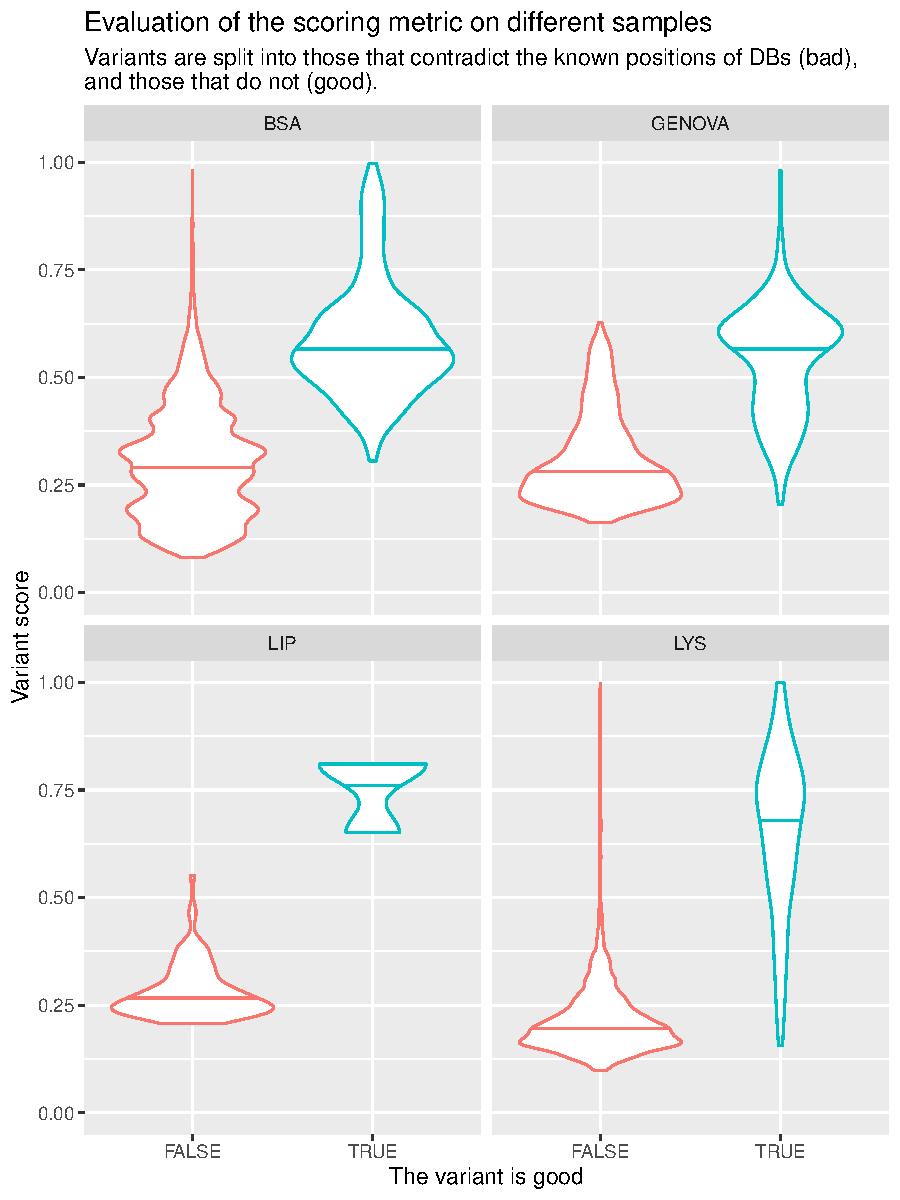
\includegraphics[width=1\linewidth]{img/scoring-metric-evaluation.pdf}
  \caption{Scoring metric evaluation on datasets from four different samples. Individual datapoints represent different assigned variants, that are grouped based on whether they contradict expert knowledge about DB positions. The boxplots illustrate that the separation is usually relatively good, but as we can see from the datapoints, there are still a lot of (in theory) nonexsting variants with a high score. This can partly be attributed to DB scrambling. The lack of data in the LIP sample is explained in the text. (BSA = bovine serum albumin, LYS = lysosyme, LIP = lipase, GENOVA = an in-silico generated ovalbumin dataset)}\label{fig:scoring-metric}
\end{figure}


\paragraph{Disulfide bond characterisation} The complete analysis was performed on three proteins, namely LYS, LIP, and GENOVA\@. In all three cases, the samples were analysed in a two step process. The analysis was first run with vanilla settings. If there was a strong evidence for a bond in the RAT data, the bond was deemed to be prone to generating false positive signals. Its weight has been adjusted to 0.1, or 0.8, depending on the strength of its RAT evidence, and the analysis was run again.

The results provided in this thesis are already post-adjustment, and can bee seen on the following figures: \Cref{fig:lys} (lysosyme, LYS), \Cref{fig:lip} (lipase, LIP), and \Cref{fig:genova} (in-silico generated ovalbumin, GENOVA). The top row shows data from RAT samples, the bottom shows data from AT samples, the left column shows the theoretical positions of the cysteine alkylations and disulfide bonds, and the right column shows the evidence we have gathered from the assigned fragments and variants. Alkylation evidence is illustrated by a border around the cysteine. Only precursor and fragment assignments that had an error of 10ppm or below were considered; we also allowed at most 2 dissociation events during fragmentation, and at most three segments in the precursor.


\begin{figure}
  \centering
  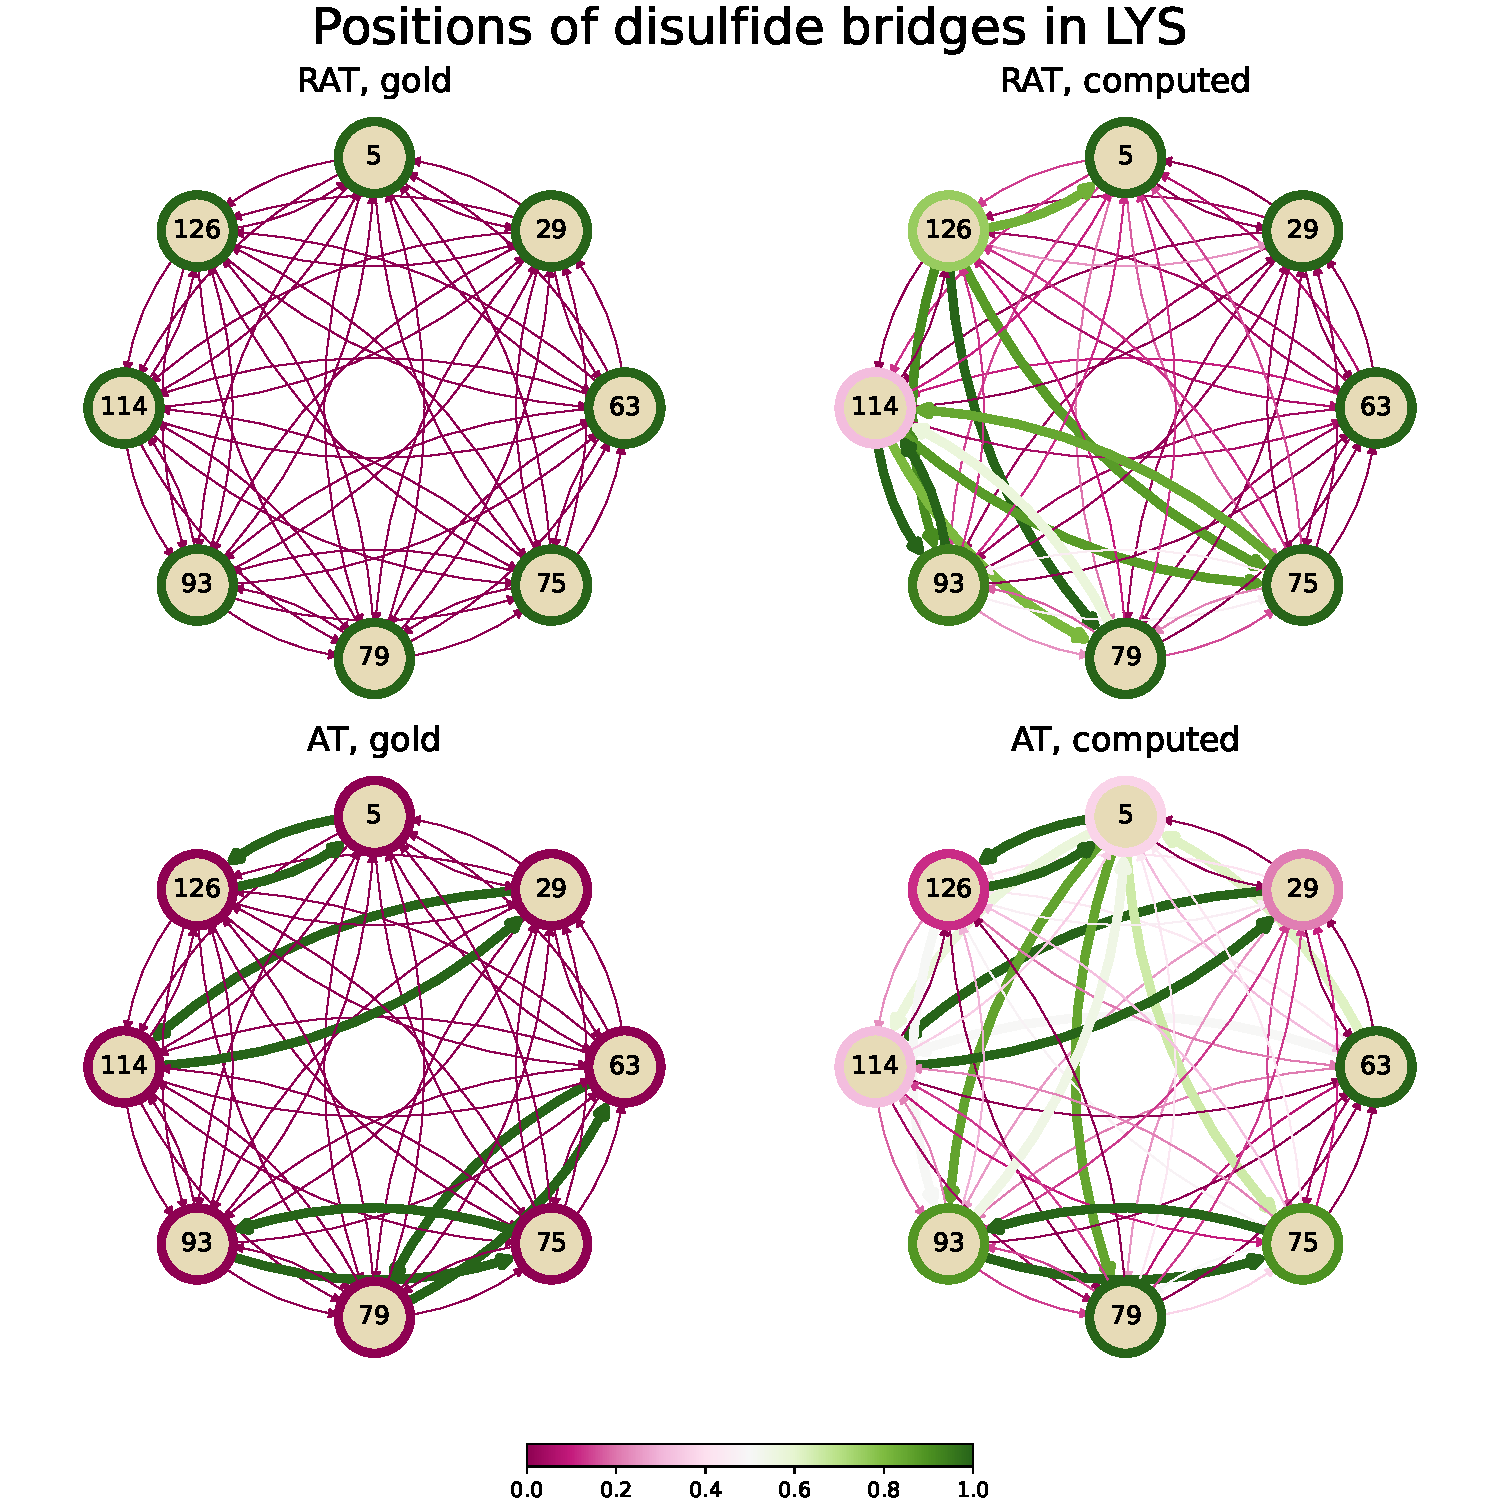
\includegraphics[width=1\linewidth]{img/lys.pdf}
  \caption{The evidence for positions of DBs and alkylations in lysosyme, weighted by variant score, and normalised. There are quite a few false positives, though not as many as to overpower all the true evidence. The bonds \((5, 126)\) and \((29, 114)\) are quite clearly visible. We can safely ignore the other directed edges stemming from 5, because their scores are relatively low compared to \((5, 126)\), and because they are not bidirectional --- that means that the supposed bond-partners are seen more commonly in other configurations. The presence of the bond \((75, 93)\) is not so clear-cut --- we also have strong signals about the cysteines being alkylated. This varrants further investigation. Finally, the evidence for bond \((63, 79)\) is practically not present, and both cysteines were deemed as alkylated.}\label{fig:lys}
\end{figure}

% TODO Doplnit přesné počty spekter

\paragraph{Lysosyme} From almost 14,000 individual spectra, 1,668 have been assigned at least one precursor. Out of the 2,219 total assigned precursors, 1,985 have generated a variant in which at least one fragment matched a peak in the spectra. Most of generated variants have in some shape or form diverged from the expert knowledge of where the bons and alkylations should be present. However, thanks to the use of our scoring metric, we have successfully identified three of the four lysosyme disulfide bonds. The cysteine pair from the last unidentified bond has been seen only in 7 fragments whose variants did not contradict our knowledge about bonds, compared for example to the 2,534 fragments of the bond \((5, 126)\). We are not sure what caused this disparity, and the causes should be more deeply investigated in the future.


\begin{figure}
  \centering
  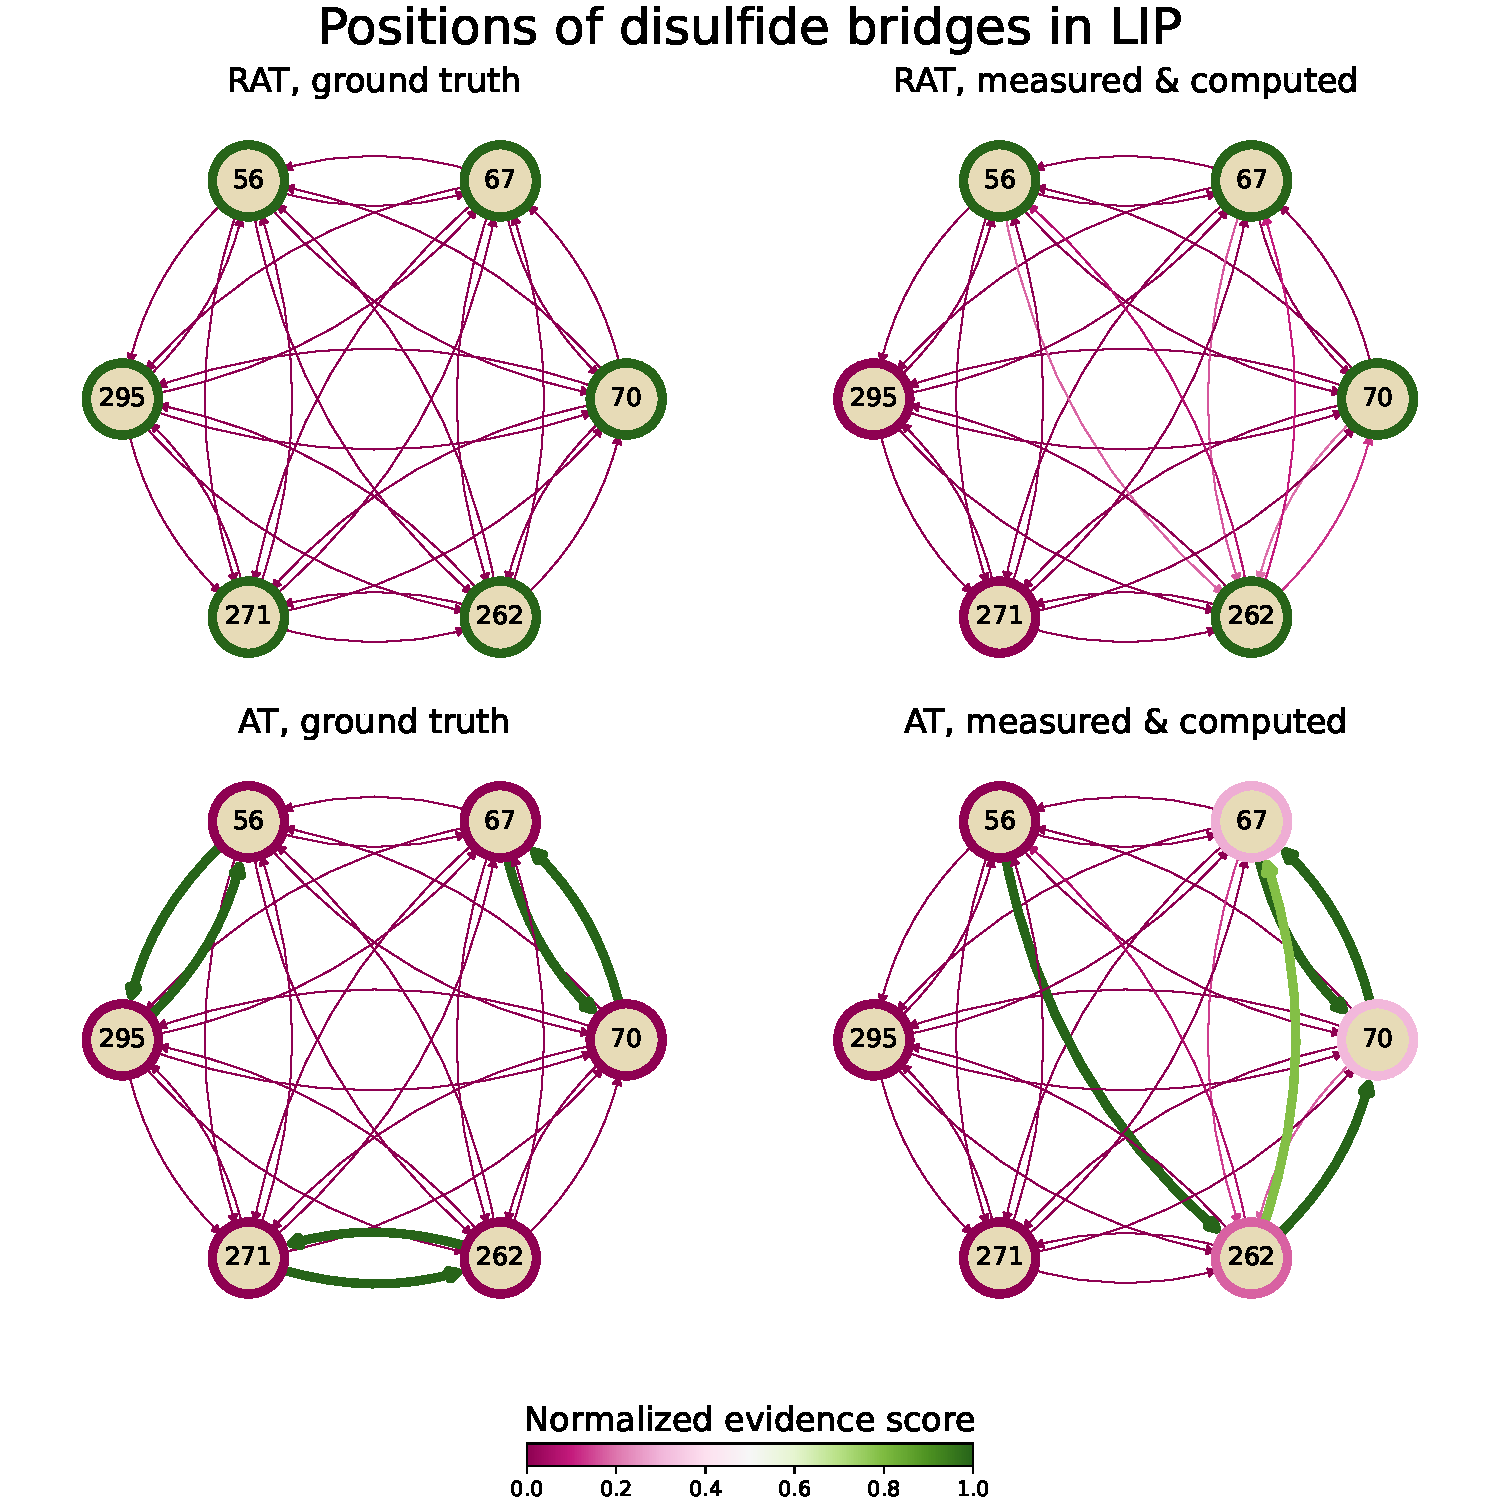
\includegraphics[width=1\linewidth]{img/lip.pdf}
  \caption{The evidence for positions of DBs and alkylations in in-silico generated ovalbumin, weighted by variant score, and normalised. No fragments containing cysteines 271 and 295 have been assigned (neither in alkylated form, nor as a part of any disulfide bond); this leads us to believe that part of the data has been lost, or otherwise damaged.}\label{fig:lip}
\end{figure}

% TODO and also to compare our assignments of simple peptides without DBs  to MSGF+\cite{kim2014ms}, a state-of-the art mass spectrometry database search tool. Přidat MSGF+, ale nejdřív ho otestovat na LIP.

\paragraph{Lipase} As is evident from the metric evaluation plot (\Cref{fig:scoring-metric}), there has been a lot less data for lipase than for the other proteins. From almost 12,000 individual spectra, only 67 have been assigned a precursor, compared to over 2,000 in lysosyme. This major disparity inspired us to construct our own control dataset. We have found that our algorithms were very prone to producting false positives, and had produced close-to-zero false negatives. Based on this fact we have concluded that a part of the lipase data has been lost, or that the data have been damaged in some uknown way. Despite these problems, Dibby successfully identifies one out of three disulfide bonds that are present in the protein.


\begin{figure}
  \centering
  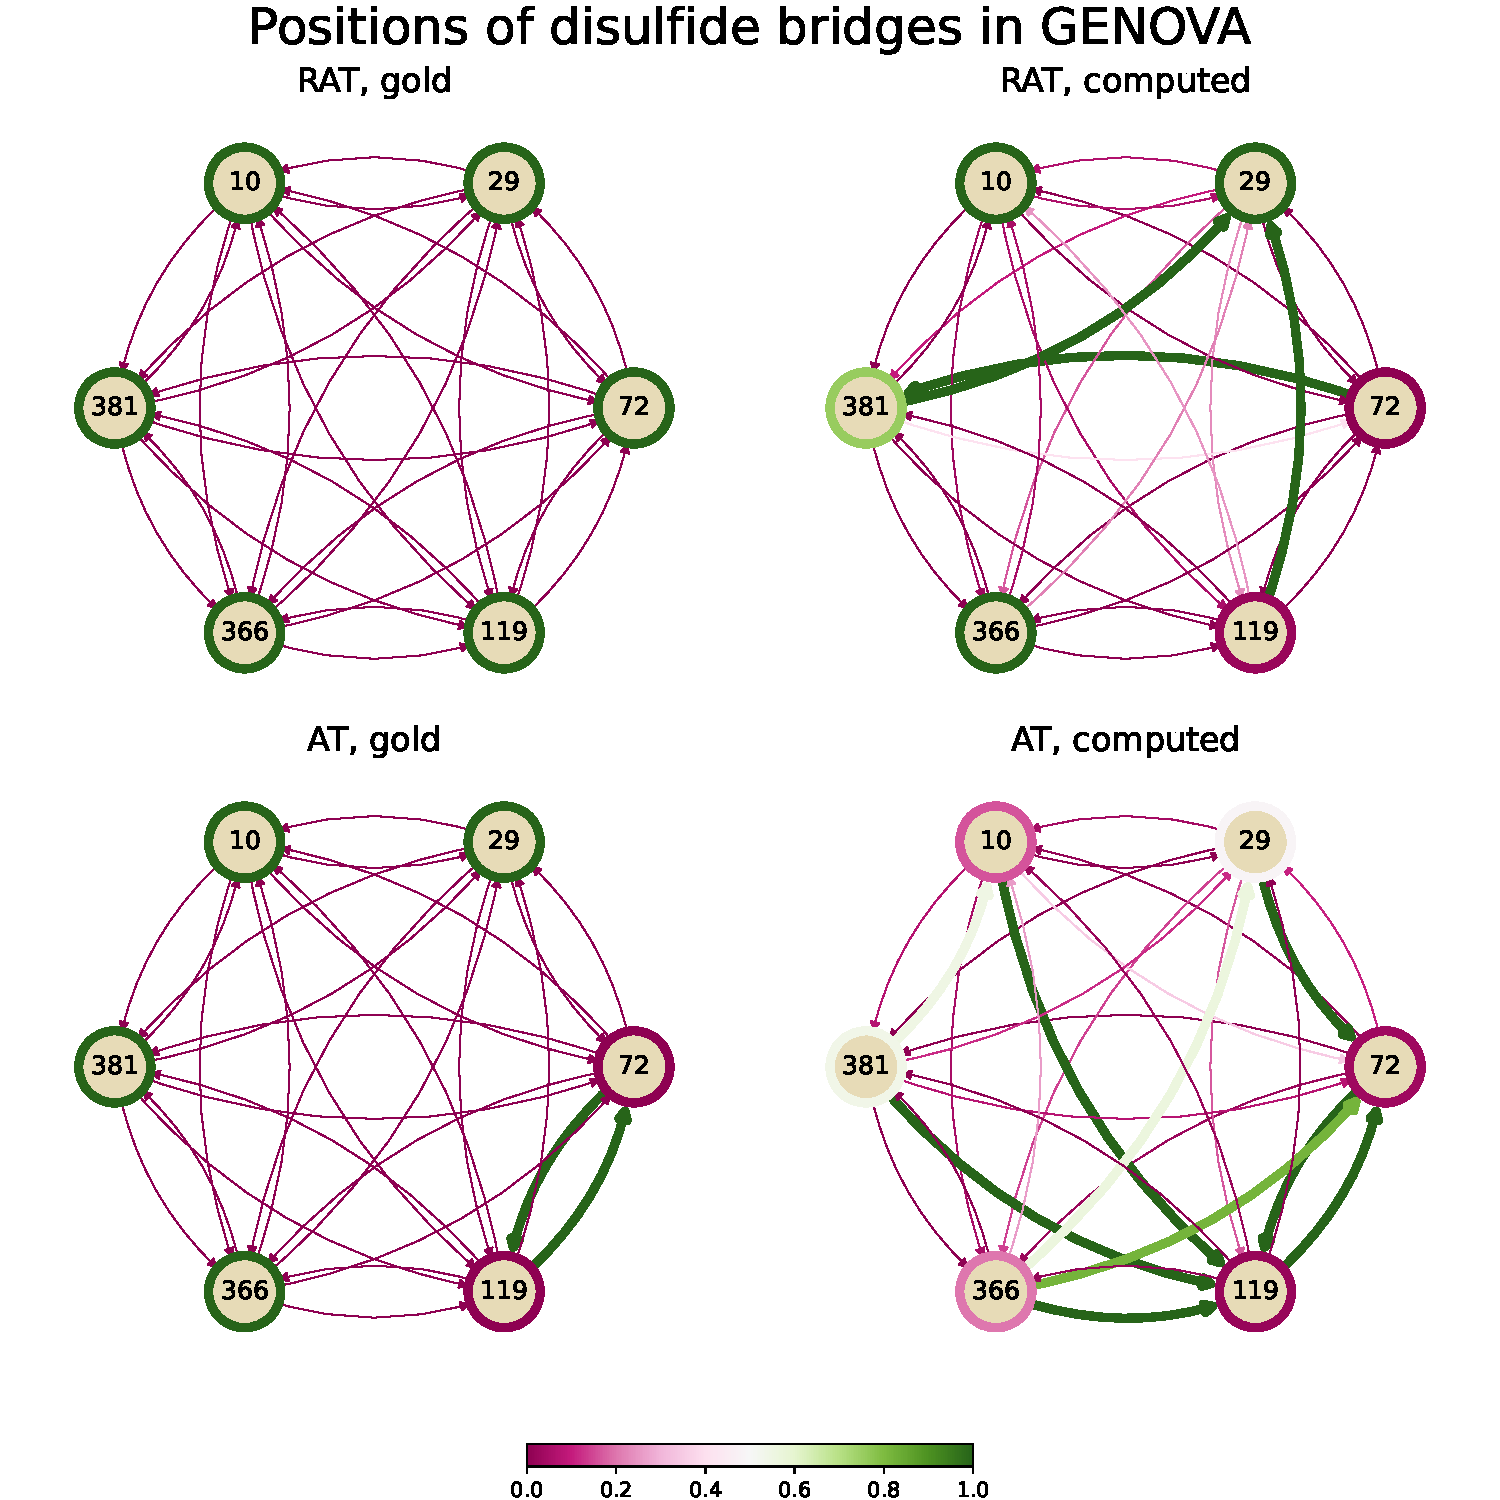
\includegraphics[width=1\linewidth]{img/genova.pdf}
  \caption{The evidence for positions of DBs and alkylations in lipase, weighted by variant score, and normalised. Although there are some false positives, leading mainly to cysteine 119, the only confirmed bidirectional bond is \((72, 119)\). }\label{fig:genova}
\end{figure}

To conclude, DB scrambling during sample preparation has proven to be a challenge, as did some ``hotspot'' cysteines that generated a lot of false signals. Despite these obstacles, we have successfully identified the majority of disulfide bonds in lysosyme, all of the bonds in our generated control, and one third of the bonds in lipase. The visualisation requires rather heavy manual interpretation, and the differential analysis step is still not automated, these two things could be made better.
